\documentclass{beamer}

\usepackage{amsmath}
\usepackage{amsfonts}
\usepackage{amssymb}
\usepackage{listings}
\usepackage{graphicx}
\usepackage{tikz}

\graphicspath{{../}}

\usetheme{default}
\useinnertheme{rectangles}
\useoutertheme{default}

\beamerdefaultoverlayspecification{<+->}

\setbeamertemplate{navigation symbols}{}

\definecolor{kcpc-bg}{RGB}{250,250,250}
\definecolor{kcpc-text}{RGB}{20,20,20}
\definecolor{kcpc-muted}{RGB}{90,90,90}
\definecolor{kcpc-red}{RGB}{176,0,0}

\setbeamercolor{background canvas}{bg=kcpc-bg}
\setbeamercolor{normal text}{fg=kcpc-text}
\setbeamercolor{frametitle}{fg=kcpc-text,bg=kcpc-bg}
\setbeamercolor{title}{fg=kcpc-text}
\setbeamercolor{subtitle}{fg=kcpc-muted}
\setbeamercolor{structure}{fg=kcpc-red}

\setbeamerfont{title}{series=\bfseries,size=\Large}
\setbeamerfont{frametitle}{series=\bfseries,size=\large}

\setlength{\parskip}{0.4em}

\setbeamertemplate{itemize item}{$\rightarrow$}
\setbeamertemplate{itemize subitem}{$\rightarrow$}

\setbeamertemplate{headline}{
    \vspace{0.2cm}
    \hspace{0.2cm}
    \textcolor{kcpc-muted}{\small\insertsection}
    \hfill
}

\setbeamertemplate{footline}{
    \hspace{0.2cm}
    \textcolor{kcpc-muted}{\small KCPC}
    \hfill
    \vspace{0.3cm}
}

\setbeamertemplate{background}{
    \begin{tikzpicture}[remember picture,overlay]
        \node[
            opacity=0.035,
            at=(current page.center)
        ] {
            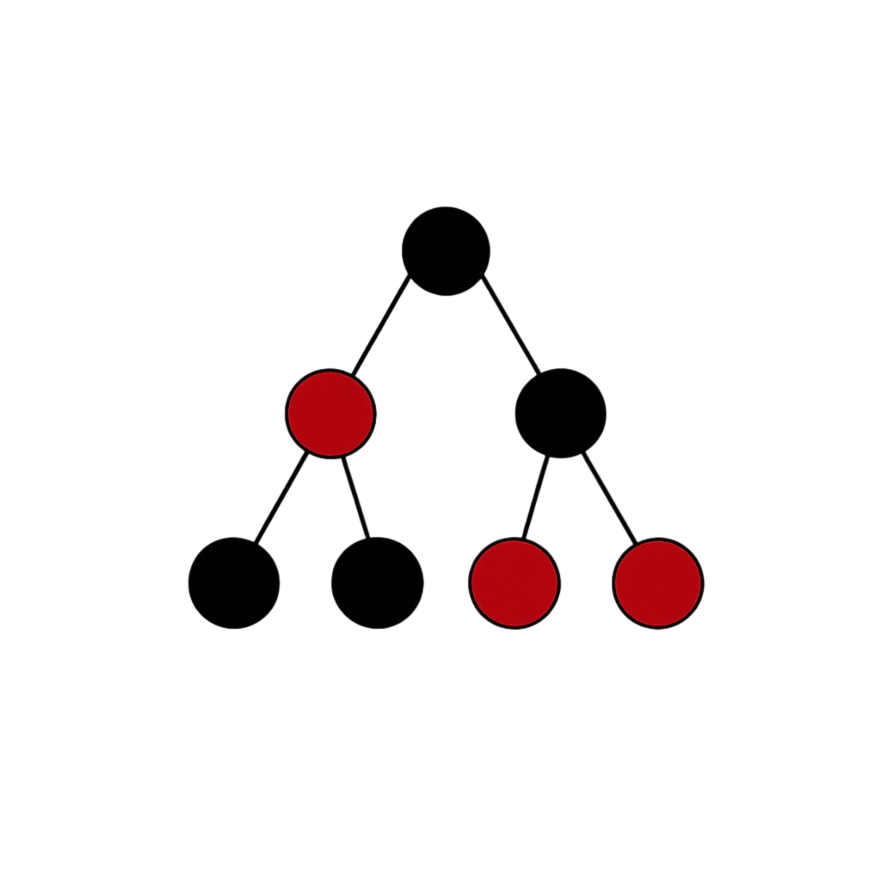
\includegraphics[width=0.55\paperwidth]{kcpc-logo.png}
        };
    \end{tikzpicture}
}

\AtBeginSection[]{
    \begin{frame}[plain]
        \vfill
        \centering
        {\Large\bfseries \insertsection}
        \vfill
    \end{frame}
}

\title{Mathematical Problem Solving II}
\subtitle{Advanced Topics and Algorithmic Thinking}
\author{KCPC}
\date{Week 2 Advanced Slides}

\begin{document}

\begin{frame}
    \titlepage
\end{frame}

\begin{frame}{Overview}
    \tableofcontents
\end{frame}

\begin{frame}{About This Deck}
    \pause
    \begin{itemize}
        \item This deck contains optional extensions beyond the core
            Week 2 heuristic methods.
        \item Use it after the main Week 2 slides or as follow-up material.
        \item Matching exercises and solutions are in the advanced sections
            of the Week 2 problem and solution sheets.
    \end{itemize}
\end{frame}

\section{Advanced Logic And Common Knowledge}

\begin{frame}{Logic Beyond Two Doors}
    \pause
    \begin{itemize}
        \item Common knowledge is what everyone knows, everyone knows
            everyone knows, and so on.
            \begin{itemize}
                \item Public announcements change the state of knowledge.
                \item Reasoning may depend on ``I know that you know
                    that I know...''
                \item Deductions continue until no possible worlds
                    can be eliminated.
            \end{itemize}
    \end{itemize}
\end{frame}

\begin{frame}{Worked Example: Muddy Children (Public Announcement)}
    $n$ children play outside. $k$ of them have mud on their foreheads.
    Each sees the others but not themselves.

    Father announces: ``At least one of you has mud.'' Then he
    repeatedly asks: ``Does anyone know their own state?''

    What happens?
\end{frame}

\begin{frame}{Solution: Muddy Children}
    \pause
    \begin{itemize}
        \item Use induction on the number of muddy children $k$.
        \item If $k=1$: that child sees no mud, knows they must be the
            one. Answers yes on round 1.
        \item If $k=2$: each sees one muddy child. If I were clean, the
            other would see 0 and answer on round 1. They don't. So I must
            be muddy. Both answer on round 2.
        \item Induction: if $k$, all $k$ answer on round $k$.
    \end{itemize}
\end{frame}

\section{Advanced Invariants And Monovariants}

\begin{frame}{Generalising Invariants}
    \pause
    \begin{itemize}
        \item An invariant can be a number, parity, polynomial, vector
            modulo $m$, or potential function.
            \begin{itemize}
                \item Modulo invariants track values mod $2,3,4,\ldots$
                \item Polynomial invariants encode several quantities at once.
                \item Potential functions never increase or never decrease.
                \item Several invariants together can prove stronger results.
            \end{itemize}
    \end{itemize}
\end{frame}

\begin{frame}{Worked Example: Grid Jumps}
    A token starts at $(0,0)$. Each move changes $(x,y)$ to either
    $(x+1,y+2)$ or $(x+2,y+1)$.

    Can the token reach $(100,100)$?
\end{frame}

\begin{frame}{Solution: Grid Jumps}
    \pause
    \begin{itemize}
        \item Track $x+y$ modulo 3.
        \item Either legal move increases $x+y$ by exactly 3.
        \item Therefore every reachable position satisfies
            $x+y\equiv0\pmod3$.
        \item At $(100,100)$, the sum is $200\equiv2\pmod3$.
        \item Hence $(100,100)$ is unreachable.
    \end{itemize}
\end{frame}

\section{Colouring And Tiling: Generalisations}

\begin{frame}{Beyond Two Colours}
    \pause
    \begin{itemize}
        \item Colouring with 3, 4, or more colours captures more structure.
            \begin{itemize}
                \item Triominoes often suggest 3-colourings.
                \item Tetrominoes can suggest 4-colourings.
                \item Colour $(i,j)$ by $(i+j)\bmod m$ or
                    $(i+2j)\bmod m$.
                \item Each tile then interacts with colour classes predictably.
            \end{itemize}
    \end{itemize}
\end{frame}

\begin{frame}{Worked Example: Deficient Board}
    A $2^n\times2^n$ board has one square removed.

    Prove that the remaining board can be tiled by L-shaped trominoes.
\end{frame}

\begin{frame}{Solution: Deficient Board}
    \pause
    \begin{itemize}
        \item Use induction on $n$.
        \item For $n=1$, the three remaining cells form one tromino.
        \item Split a larger board into four equal quadrants.
        \item Place one central tromino so each quadrant has exactly
            one missing square.
        \item Tile each smaller deficient quadrant by induction.
    \end{itemize}
\end{frame}

\section{Induction And Recursion: From Proof To Algorithm}

\begin{frame}{Induction As A Design Principle}
    \pause
    \begin{itemize}
        \item If I can solve size $n$ using a solution for size $n-1$,
            I have a recursive algorithm.
            \begin{itemize}
                \item Proof by induction $\leftrightarrow$ recursive function.
                \item Base case $\leftrightarrow$ terminating condition.
                \item Inductive step $\leftrightarrow$ recursive call.
                \item Strong induction $\leftrightarrow$ divide-and-conquer or DP.
            \end{itemize}
    \end{itemize}
\end{frame}

\begin{frame}{Worked Example: Tower Of Hanoi}
    Three pegs, $n$ disks of decreasing size. Move stack from peg A to peg C.
\end{frame}

\begin{frame}{Solution: Tower Of Hanoi}
    \pause
    \begin{itemize}
        \item Build a recursive solution from induction on $n$.
        \item Move top $n-1$ disks from A to B.
        \item Move largest disk from A to C.
        \item Move $n-1$ disks from B to C.
        \item Minimum moves: $2^n-1$ (prove by induction).
        \item The recursive structure \emph{is} the algorithm.
    \end{itemize}
\end{frame}

\section{From Mathematical Insight To Algorithmic Thinking}

\begin{frame}{The Bridge To Competitive Programming}
    \pause
    \begin{itemize}
        \item A mathematical proof often suggests an algorithm directly.
            \begin{itemize}
                \item An invariant becomes a loop invariant.
                \item Induction becomes recursion or a DP recurrence.
                \item Reduction becomes the modelling step.
                \item A proof of progress becomes a termination argument.
            \end{itemize}
    \end{itemize}
\end{frame}

\begin{frame}{Modelling A Puzzle As A Graph (Algorithmic Bridge)}
    \pause
    \begin{itemize}
        \item Many puzzles become graph reachability or shortest-path problems.
            \begin{itemize}
                \item A state completely describes the current situation.
                \item An edge represents one legal move.
                \item A solution is a path from the start to a goal state.
                \item BFS finds a path using the fewest moves.
                \item An invariant can separate disconnected components.
            \end{itemize}
    \end{itemize}
\end{frame}

\begin{frame}{Worked Example: Water Jugs As A Graph}
    Two jugs of capacities 3 and 5. Target: measure exactly 4 units.
    Allowed: fill, empty, pour.

    How can this be modelled and solved as a shortest-path problem?
\end{frame}

\begin{frame}{Solution: Water Jugs}
    \pause
    \begin{itemize}
        \item Represent a state by $(a,b)$, where
            $0\le a\le3$ and $0\le b\le5$.
        \item Add edges for filling, emptying, and pouring between jugs.
        \item Run BFS from $(0,0)$ until one coordinate is 4.
        \item One shortest route is
            $(0,0)\to(0,5)\to(3,2)\to(0,2)\to(2,0)\to(2,5)\to(3,4)$.
    \end{itemize}
\end{frame}

\begin{frame}{Greedy Choices From The Extreme Principle (Algorithmic Bridge)}
    \pause
    \begin{itemize}
        \item The extreme principle often justifies a greedy choice.
            \begin{itemize}
                \item Activity selection chooses the earliest finish time.
                \item Canonical coin change chooses the largest coin.
                \item Fractional knapsack chooses the highest value density.
                \item An exchange argument proves the choice is safe.
            \end{itemize}
    \end{itemize}
\end{frame}

\begin{frame}{Recurrence From Induction (Algorithmic Bridge)}
    \pause
    \begin{itemize}
        \item Inductive proofs directly give recurrences.
            \begin{itemize}
                \item Define $f(n)$ as the answer for size $n$.
                \item Express $f(n)$ using answers to smaller instances.
                \item Memoise or tabulate to avoid recomputation.
                \item This turns the proof into dynamic programming.
            \end{itemize}
    \end{itemize}
\end{frame}

\begin{frame}{Wrap-Up}
    \pause
    \begin{itemize}
        \item Common knowledge extends formal logical reasoning.
        \item Generalised invariants and colourings prove stronger results.
        \item Inductive proofs lead directly to recursive algorithms.
        \item Mathematical models lead to graph, greedy, and DP techniques.
    \end{itemize}
\end{frame}

\begin{frame}{Thanks for going further!}
    \begin{center}
        \Large
        \textbf{Thank you for reading and completing the extra material!}

        See ya next week!
    \end{center}
\end{frame}

\end{document}
